\chapter{Konzeption}\label{ch:konzeption}

Das Grundprinzip des entwickelten Systems basiert auf einer Abwandlung der generalisierten Hough-Transformation.
Diese wurde auf drei Dimensionen erweitert und mit mehreren Nachbearbeitungsschritten ergänzt um nicht nur Positionen sondern auch Orientierungen zu beachten.
Dabei besteht die Verarbeitungskette bis zur erfolgreichen Erkennung von Szenen aus drei grundlegenden Schritten.
Als Erstes werden über einen längeren Zeitraum von mehreren Minuten bis Stunden hinweg die erkannten Objekte gespeichert.
Dabei wird der Aufnahmezeitraum in kleinere Zeitschritte zerlegt (beispielsweise 5 Sekunden) und für jeden Zeitschritt werden die in dieser Zeit seit dem vorherigen Schritt wahrgenommenen Objekte als ein Szenenausschnitt gespeichert.
Darauf folgt die Verarbeitung aller aufgenommen Ausschnitte zu einem vollständigen Modell, diese Phase stellt das eigentliche Training dar.
Mit dem fertigen Modell werden dann bereits trainierte Szenen innerhalb einer Menge wahrgenommener Objekte erkannt.

\section{Begriffe}
Um eine einfache Beschreibung der Zusammenhänge zu ermöglichen werden hier kurz die verwendeten Begriffe definiert:
\begin{description}
  \item[Pose] \hfill \\
  Eine Pose ist eine Repräsentation einer Lage im Raum.
  Sie enthält sowohl einen dreidimensionalen Positionsvektor als auch ein Quaternion zur Beschreibung der Orientierung.

  \item[Objekt] \hfill \\
  Ein Objekt ist eine allgemeine Repräsentation eines von den Objekterkennern erkannten Gegenstandes.
  Beispielsweise eine Tasse, ein Tisch oder ähnliches.\\
  Es muss mindestens folgende Attribute enthalten:
  \begin{itemize}
    \item Typ
    \item Identifikator
    \item Position in drei Dimensionen
    \item Orientierungen in drei Dimensionen
    \item Gewicht
  \end{itemize}

  Der Typ bezeichnet hierbei die generelle Klasse des Objektes, beispielsweise "`Tasse"'.
  Der Identifikator dagegen ist nicht zwangsweise eine Eigenschaft des realen Gegenstandes, sondern kann auch separat als Annotation den Trainingsdaten beigefügt werden.
  Sollten beispielsweise zwei identisch aussehende Tassen gleichzeitig erkannt werden (gleicher Objekttyp), so können diese mit Hilfe eines Identifikators als "`Tasse 1"' und "`Tasse 2"' unterschieden werden.
  Identifikatoren lösen damit Probleme in der Unterscheidbarkeit identischer aussehender Objekte innerhalb einer Szene.
  Das Gewicht eines Objektes ist ein Zahlenwert der festlegt, wie wichtig ein Objekt innerhalb einer Szene ist.
  Besitzen beispielsweise in einer Szene aus 4 Objekten alle Objekte das Gewicht 1, so wird die Erkennungssicherheit durch das Fehlen eines Objektes um 1/4 verringert.

  \item[Objektmenge] \hfill \\
  Eine Objektmenge enthält eine Anzahl an zu der Szene gehörenden Objekten.
  Dabei muss jede Kombination aus Objekt-Typ und Objekt-Identifikator jeweils eindeutig sein.
  Das heißt, es darf keine zwei Objekte in der Menge mit identischem Typ und Identifikator geben.
  Die Objektmenge enthält damit die bei der Aufnahme innerhalb eines Zeitschrittes gesehenen Objekte.

  \item[Szene] \hfill \\
  Eine Szene bezeichnet ein Objekte oder eine Konstellation mehrerer Objekte, zusammen mit der zeitlichen Änderung ihrer Position und Orientierung .
  Sie ergibt sich aus der Zusammenfassung aller Objektmengen über die Aufnahmedauer.
  Zu jeder Szene gehört ein erwartetes Gewicht, welches bestimmt wird aus dem durchschnittlichen Gesamtgewicht der Objektmengen.
  Das Gesamtgewicht einer Objektemenge bezeichnet dabei lediglich die Summe der Gewichte alle enthaltenen Objekte.

  \item[Spur] \hfill \\
  Die Spur eines Objektes enthält, zeitlich sortiert, alle Vorkommen eines Objektes innerhalb aller zu einer Szene gehörenden Objektmengen.
  Sie stellt damit die zeitliche Änderung der Position und Lage eines Objektes dar.
  Sollte ein Objekt in einem Zeitschritt nicht erkannt worden sein, ist an der entsprechende Stelle der Spur der Wert $null$ verzeichnet.

  \item[Heuristik] \hfill \\
  Eine Heuristik ist ein Algorithmus, welcher aus einer Menge von Spuren einen gewichteten Vorschlag generiert und aussagt, wie stark zwei bestimmte Spuren innerhalb der Menge zusammenhängen.
  Das Zusammenhangskriterium kann dabei Situationsabhängig gewählt werden, beispielsweise "`Objekte der Spur A sind immer an der linken Seite von Objekten der Spur B"'.
  Er implementiert damit die Funktion:\\
  \{Menge von Spuren\} $\rightarrow$ ($Spur_1$, $Spur_2$, Konfidenz des Vorschlags)

  \item[Vote] \hfill \\
    Ein Vote ist eine Beschreibung der Transformation von einer Objektpose zu einer Referenzpose und eine entsprechende Rücktransformation.
    Zusätzlich enthält es den Typ und den Identifikator des Objektes, sowie den Szenennamen, für den es eine "`Stimme"' abgibt.

  \item[Angewandtes Vote] \hfill \\
    Ein angewandtes Vote ist ein Container, welcher ein Objekt und ein Vote, zusammen mit der Referenzpose, speichert.
    Die Referenzpose erhält man, indem man die Objektpose, mit der im Vote gespeicherten Transformation, transformiert.
    Zusätzlich enthält es ein Gewicht, welches sich aus der Differenz des Gewichtes des Objektes und dem erwarteten Gesamtgewicht der zum Vote gehörenden Szene ergibt.
 
  \item[Erkennungsergebnis] \hfill \\
    Ein Erkennungsergebnis ist ein Container, welcher das Erkennungsresultat kapselt.
    Es beinhaltet den zugehörigen Szenennamen, die eingeschlossenen Objekte aus der Eingabemenge sowie einen Konfidenzwert und die Referenzpose der erkannten Szene.

\end{description}

\section{Aufnahme}

Da Implicit Shape Models auf einer Wiedererkennung im voraus aufgezeichneter geometrischer Konstellationen beruhen, ist es notwendig Beobachtungsdaten aufzuzeichnen.
Dies erfolgt im Rahmen der Szenenerkennung indem eine reale Szene über mehrere Minuten oder Stunden hinweg beobachtet wird.
Dabei werden die Sensordaten permanent von Objekterkennern verarbeitet, woraus ein konstanter Fluss an erkannten Objekten innerhalb der wahrgenommen Szene resultiert.
Diese von den Objekterkennern bereitgestellten Objekte werden wiederholt über einen kurzen Zeitraum (beispielsweise 5 Sekunden) hinweg aggregiert und zu einer Objektmenge zusammengefasst.
Die entstandenen Objektmengen werden mit dem Szenennamen annotiert und in einer Datenbank für das spätere Training abgelegt.

\section{Training}

\subsection{Implicit Shape Model Generierung}

Für die Generierung der Implicit Shape Models wird eine auf den Anwendungsfall spezialisierte Auslegung der generalisierten Hough-Transformation benutzt.
Um zu verstehen, was in diesem Verfahren berechnet wird, ist es notwendig zuerst das Konzept eines Votes zu verstehen.

\subsubsection{Vote}\label{ch:vote}

Ein Vote repräsentiert im Allgemeinen eine Transformation von einer Objektpose zu einer Referenzpose und eine entsprechende Umkehrtransformation.

Es beinhaltet zwei Drehquaternionenpaare zusammen mit einem Radius als Skalierungsfaktor, sowie dem zugehörigen Szenennamen, Objekttyp und Objektidentifikator(ID).
Jedes Quaternionenpaar besteht aus einem Quaternion zur Drehung der aktuellen Objektorientierung in Richtung eines (Referenz-)Punktes und einem Quaternion zur Drehung der aktuellen Objektorientierung in die Orientierung eines anderen Objektes.
Das erste Paar stellt dabei die Transformation von Objekt zu Referenzpose und das zweiter Paar die Transformation von Referenzpose zu Ursprungsobjekt dar.
Diese Darstellung ermöglicht eine flexible Anwendung der Transformationen.
Ist es beispielsweise nur notwendig aus einer Objekt-Vote-Kombination den Zielpunkt des Votes zu errechnen, so muss man lediglich das aktuelle Objekt mit dem Richtungsquaternion drehen und den daraus resultierenden Einheitsvektor in Richtung des Zielpunktes mit dem Radius multiplizieren.
Sollte eine komplette Lagetransformation erforderlich sein, führt man den ersten Teil des Verfahrens aus um den neuen Lagepunkt zu erhalten, nach transformiert man lediglich das originale Lagequaternion mit dem Quaternion für die Lageänderung und erhält ein rotiertes und verschobenes Objekt.
Dieses Verfahren ist angelehnt an das von \citeauthor{trove.nla.gov.au/work/45506311} präsentierte Verfahren\betterfootcite{trove.nla.gov.au/work/45506311} und bietet Vorteile beim Speicheraufwand sowie einer Vermeidung von kardanischen Blockaden bei der Verwendung von Quaternionen im Gegensatz zu 4x4 Transformationsmatrizen.

\begin{figure}
  \centering
  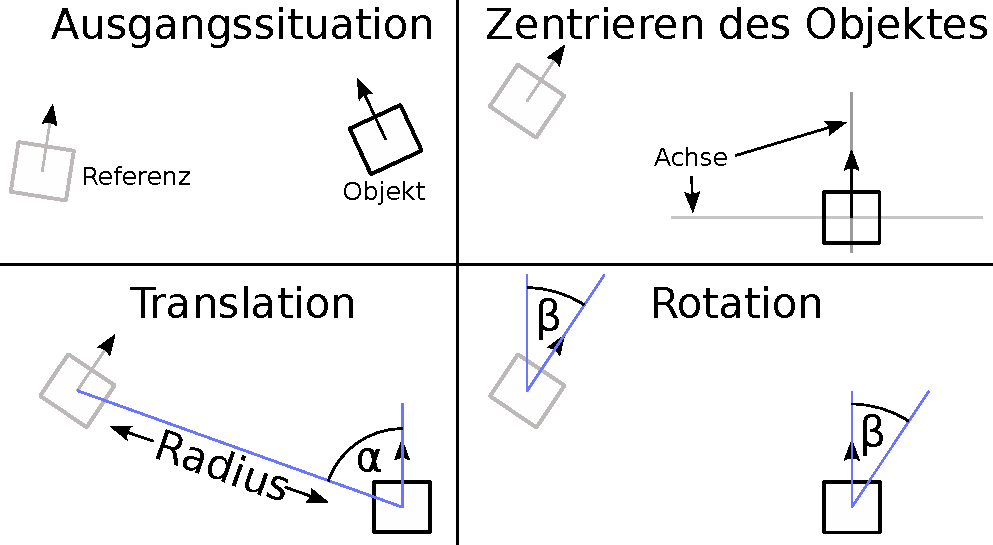
\includegraphics[width=0.7\textwidth]{./bilder/votes.pdf}
  \caption{Errechnung der Votetransformationen in 2 Dimensionen}\label{fig:votes}
\end{figure}

Die Berechnung eines Votes ist beispielhaft in 2 Dimensionen in Abbildung \vref{fig:votes} dargestellt und erfolgt durch das folgende Verfahren:

Als Erstes wird das votende Objekt und die Referenzpose in ein Koordinatensystem $\Gamma_O$ transformiert, sodass das votende Objekt im Ursprung liegt und die durch die Orientierung des Objektes gegeben lokalen Achsen an den Koordinatensystemachsen ausgerichtet sind.
Dafür definieren wir zunächst die Einheitsquaternionen $\mathbf{q}_o$ für das Orientierungsquaternion des votenden Objektes und $\mathbf{q}_r$ für das Orientierungsquaternion der Referenzpose sowie einen Vektor $\mathbf{v}_{otr}$ von der Objektposition zur Position der Referenzpose.
Dann wird $\mathbf{v}_{otr}$ in den Vektor $\mathbf{v}_{otr}'$ in $\Gamma_O$-Koordinaten transformiert.

\begin{equation}
  \begin{array}{rcl}
    \mathbf{v}_{otr}' & = & \mathbf{q}_o \mathbf{v}_{otr} \mathbf{q}_o^{-1}
  \end{array}
\end{equation}

Aus diesem Vektor $\mathbf{v}_{otr}'$ kann nun das Drehquaternion $\mathbf{q}_{otr}$ für die Drehung des Objektes berechnet werden, sodass der Blickvektor des Objektes in Richtung der Referenzpose zeigt.

\begin{equation}
  \begin{array}{rcl}
    \mathbf{v}_0 & = & \mathbf{v}_{otr}' / \|\mathbf{v}_{otr}'\|\\
    \mathbf{v}_1 & = & \begin{rcases}{(1, 0, 0)}^T\end{rcases} \text{Standard-Blickrichtungsvektor}\\
    \mathbf{a} & = & \mathbf{v}_0 \times \mathbf{v}_1\\
    w & = & 1 + \mathbf{v}_0 \cdot \mathbf{v}_1\\
    \mathbf{t} & = & {(\mathbf{a_x},\mathbf{a_y},\mathbf{a_z},w)}^T\\
    \mathbf{q}_{otr} & = & t / \|t\|
  \end{array}
\end{equation}

Zur Berechnung des Drehquaternions $\mathbf{q}_{otrp}$ zwischen der Orientierung des Objektes und der Orientierung der Referenzpose wird lediglich die Standardquaternionenrotation benötigt.

\begin{equation}
  \begin{array}{rcl}
    \mathbf{q}_{otrp} & = & {\mathbf{q}_o}^{-1} \mathbf{q}_r
  \end{array}
\end{equation}

Dieses Verfahren wird analog wiederholt, jedoch nicht aus Perspektive des Objektes, sondern aus Perspektive der Referenzpose um einen vollständigen Satz aus zwei Quaternionenpaaren für die Transformation zwischen den Posen zu erhalten.

\subsubsection{Algorithmus zur Generierung von Implicit Shape Models}

Der in Algorithmus \vref{algo:ism-generierung} dargestellte Ablauf implementiert eine an den Anwendungsfall angepasste Implementierung der Generierung eines Implicit Shape Models.
Wie im Voraus schon erwähnt, wird das Modell aus einer zeitlich sortierten Menge von Objektmengen sowie einem Szenennamen generiert.
Der Szenenname wird dabei vom Benutzer gegeben, da es sich um einen überwachten Lernvorgang handelt.
Das fertige Modell wird in einer Datenbank abgelegt und eine Spur des gewählten Referenzobjektes für die Weiterverarbeitung zurückgegeben.

\paragraph{Referenzpuntwahl}
Als ersten Schritt des Verfahrens muss ein geeignetes Referenzobjekt ausgewählt werden.
Um dies zu vereinfachen, wird die Menge von Objektmengen $O_{MM}$ in eine Spurenmenge \textit{Spuren} der enthaltenen Objekte umgewandelt.
Es folgt die Sortierung der Spurenmenge nach zwei Kriterien, vorerst nach möglichst häufigem Auftauchen des Objektes in den Spuren, darauf folgend nach möglichst niedriger Positionsvarianz.
Damit wird sichergestellt, dass Objekte bevorzugt werden, welche bei der Erkennung eine höhere Wahrscheinlichkeit auf Wiederfindung aufweisen.
Sollten mehrere Objekt gleich häufig auftauchen, wird das Objekt bevorzugt, welches sich über den Beobachtungszeitrum am wenigsten bewegt.
Diese Bedingung hat sich in Experimenten als günstig erwiesen, da Objekte mit einer hohen Positionsvarianz auf schnell bewegte Objekte oder auf ein starkes Sensorrauschen/Erkennerrauschen hindeuten.
Da sowohl die Wahl von schnellen Objekten als auch Objekte mit einer großen Sensorrauschen bedingten Positionsvarianz vermieden werden sollen, werden statische Objekte bevorzugt.
Nachdem mit diesem Verfahren eine Spur ausgewählt wurde, werden dessen Objekttyp und Objektidentifikator vermerkt, um für die spätere Wiedererkennung des Referenzobjektes benutzt werden zu können.

\paragraph{Generierung des ISM}

\begin{algorithm}
  \caption{Generierung eines Implicit Shape Models}
  \small
  \label{algo:ism-generierung}
  \begin{algorithmic}[1]
    \Require Sortierte Menge von Objektmengen $O_{MM}$, Szenenname $SName$\;
    \Ensure Referenzspur\;
    \State Referenzspur $\gets \{\}$\;
    \State Spuren $\gets$ Umwandlung von $O_{MM}$ in Menge von Spuren\;
    \State ZielRefTyp, ZielRefID $\gets$ \parbox[t]{\dimexpr\linewidth-140pt\relax}{
      Finde Typ/ID für am häufigsten auftauchendes Objekt. Falls nicht eindeutig, bevorzuge weniger Positionsvarianz.}\strut\;
    \ForAll{$O_M \in O_{MM}$}
      \State Referenzpose $\gets$ null\;
      \If{$\exists o \in O_M : o.\text{Typ} = \text{ZielRefTyp} \wedge o.\text{ID} = \text{ZielRefID}$}
        \State Referenzpose $\gets o.\text{Pose} :$ \parbox[t]{\dimexpr\linewidth-140pt\relax}{$o \in O_M \wedge $\\
            $o.\text{Typ} = \text{ZielRefTyp} \wedge$\\
            $o.\text{ID} = \text{ZielRefID}$}\strut\;
      \ElsIf{$\left| O_M \right| > 0$}
        \State Referenzpose $\gets O_M[1].\text{Pose}$\;
      \Else
        \State Füge null zu Referenzspur hinzu\;
        \State continue\;
      \EndIf
      \ForAll{$o \in O_M$}
        \State Vote $\gets$ Berechne Vote von $o$ nach Referenzpose\;
        \State Vote.Szenenname $\gets$ SName\;
        \State Vote.Typ $\gets o.\text{Typ}$\;
        \State Vote.ID $\gets o.\text{ID}$\;
        \State Speichere Vote in Datenbank\;
      \EndFor
      \State Referenzobjekt $\gets$ Objekt mit: \parbox[t]{\dimexpr\linewidth-\algorithmicindent-\algorithmicindent\relax}{
        Typ $\gets$ SName\\
        Pose $\gets$ Referenzpose\\
        Gewicht $\gets \sum \{o.\text{Gewicht} | o \in O_M\}$
      }\strut\;
      \State Füge Referenzobjekt zu Referenzspur hinzu\;
    \EndFor
    \State ErwartetesGewicht $\gets \left[ \frac{\sum \{o.\text{Gewicht} | o \in \text{RefernzSpur} \wedge o \neq \text{null}\})}{\left| O_{MM} \right|} \right]$
    \State Speichere Szene in Datenbank mit: \parbox[t]{\dimexpr\linewidth-\algorithmicindent\relax}{Name $\gets$ SName\\
    ErwartetesGewicht $\gets$ ErwartetesGewicht}\strut\;
    \State \Return Referenzspur\;
  \end{algorithmic}
\end{algorithm}

Es folgt die eigentliche ISM-Generierung.
Zunächst wird die Variable \textit{ReferenzSpur} definiert, welche später zurückgegeben werden soll und die Spur des Referenzobjektes enthält.
Daraufhin muss über jede Objektmenge $O_M$ in $O_{MM}$ iteriert werden.
Zuerst wird ermittelt, ob es in der aktuellen Objektmenge $O_M$ ein Objekt gibt, welches den vorher gewählten Objekttyp und Identifikator des Referenzobjektes besitzt.
Wenn dies der Fall ist, dann wird die Pose dieses Objektes als Referenzpose vermerkt.
Sollte es kein passendes Objekt in $O_M$ geben, jedoch $O_M$ nicht leer sein, so wird ein beliebiges Objekt aus $O_M$ für die Referenzpose benutzt.
Sollte $O_M$ leer sein, so wird \textit{ReferenzSpur} ein Nullobjekt hinzugefügt um eine leere Stelle zu dokumentieren und es wird an das Ende der Schleife gesprungen um ohne weitere Aktionen zur nächsten Iteration zu gelangen.
Die Wahl einer beliebigen Referenzpose im vorherigen Schritt ist dadurch gerechtfertigt, dass ein ISM nicht zwangsweise schlechtere Ergebnisse bei Verwendung eines zufälligen Referenzpunktes liefert.
Dabei ist eine zufällige Wahl mit geringerer Erkennungsrate in jedem Fall einer nicht vorhandenen Erkennung vorzuziehen.

Es folgt die Generierung der einzelnen Votes für das Implicit Shape Model.
Dafür wird über die Objektmenge $O_M$ iteriert.
Für jedes Objekt wird ein Vote zu der im voraus bestimmten Referenzpose nach dem Verfahren in Abschnitt \vref{ch:vote} generiert, mit Szenenname, Objekttyp und Objektidentifikator annotiert und das Vote in der Datenbank gespeichert.
Nach dem Ende der Iteration wird aus der Referenzpose ein Referenzobjekt generiert, welches als Typ den Szenennamen, als Pose die Referenzpose und als Gewicht die Summe aller Objektgewichte in $O_M$ trägt.
Dieses Referenzobjekt wird dann der Referenzspur hinzugefügt.
Wenn dieser Ablauf für alle Objektmengen in $O_{MM}$ abgeschlossen wurde, wird in der Datenbank ein Eintrag für die gelernte Szene hinterlegt.
Dieser enthält den Szenenamen und das erwartete Gewicht aller Objekte in einer Szene.
Zur Bestimmung des erwarteten Gewichtes wird erst die Summe aller Gewichte der Objekte in der Referenzspur berechnet.
Dieses wird dann durch die Mächtigkeit von $O_{MM}$ geteilt und kaufmännisch gerundet.
Am Ende des Verfahrens wird die erstellte Referenzspur zurückgegeben.

\subsection{Heuristiken}

Die Heuristiken bilden in unserem System die zentralen Komponenten zum erkennen von dynamischen Zusammenhängen.

Zur Lösung des in Abschnitt \vref{ch:ISM-Probleme} dargestellte Vertauschungsproblem wurde eine Heuristik definiert um direktionale Zusammenhänge innerhalb dynamischer Szenen zu erkennen.
Der entwickelt Ansatz basiert auf der Erweiterung bekannter ISM Verfahren um die Erkennung von winkelabhängigen Zusammenhängen.
Ein alltägliches Beispiel eines solchen Zusammenhanges ist eine typische "`A steht immer rechts von B"' Beziehung.
Die Heuristiken extrahieren diesen Zusammenhang aus einer gegebenen Spurmenge und geben als Ergebnis ein Spurenpaar zusammen mit einem Konfidenzwert oder nichts zurück.
Wurde ein Spurenpaar mit genügender Konfidenz erkannt, wird es als ein separates ISM trainiert und in der Eingabemenge durch die Spur des erzeugten Unter-ISMs ersetzt.

Es ist wichtig festzustellen, dass Heuristiken nicht nur auf diesen Zusammenhang beschränkt sind, sondern beliebige zusammenhänge erfassen können.
Für die Lösung aller im Experiment auftretenden Probleme war jedoch die direktionale Heuristik ausreichend.

\subsubsection{Direktionale Heuristik}\label{ch:heuristik}

\begin{algorithm}
  \caption{Direktionale Heuristik}
  \small
  \label{algo:heuristik-direktional}
  \begin{algorithmic}[1]
    \Require Spurenmenge $M_S$\;
    \Ensure Spurenpaar mit Konfidenz oder nichts\;
    \State Ergebnis, ErgebnisKonfidenz, ErgebnisDistanz $\gets$ null\;
    \ForAll{$S_1 \in M_S, S_2 \in M_S : S_1 \neq S_2$}
        \State $GS \gets \{ i \in \mathbb{N} | \exists a_i \neq \text{null} \wedge b_i \neq \text{null}, a_i \in S_1, b_i \in S_2 \} $\;
        \State $NGS \gets \left| GS \right| $\;
        \If{$NGS < (\left| S_1 \right| * \text{MinGemeinsamkeitsQuote})$}
            \State continue\;
        \EndIf

        \State $D \gets \sum \{\left\Vert a_i - b_i \right\Vert | i \in GS, a_i \in S_1, b_i \in S_2\}$\;
        \State $AD \gets D / NGS $\;

        \State $BR \gets 0$\; \Comment{Anzahl der Zusammenhangsbrüche}
        \State $RV \gets \text{null}$\; \Comment{Vektor von $a \in S_1$ in Richtung $a \in S_2$}
        \ForAll{$a_i, b_i | i \in GS, a_i \in S_1, b_i \in S_2$} \Comment{$i$ muss monoton steigend sein}
            \If{$RV = \text{null}$}
                \State $RV \gets $Richtungsvektor von $a_i$ nach $b_i$ in $a_i$ Koordinaten\;
                \State continue\;
            \EndIf
 
            \State $AV \gets$ Richtungsvektor von $a_i$ nach $b_i$ in $a_i$ Koordinaten\;
            \State Abweichung $\gets$ Winkelabweichung zwischen $AV$ und $RV$\;
            \If{Abweichung > Abweichungsschwellwert}
                \State $BR \gets BR + 1$\;
                \State $RV \gets AV$\;
            \EndIf
        \EndFor
        \If{$BR < (NGS * $MaxBruchverhältnis$)$}
            \State Distanz $\gets AD$\;
            \State Konfidenz $\gets BR / NGS$\;
            \State Kond$_1$ $\gets$ Ergebnis $=$ null $\vee$ Konfidenz > ErgebnisKonfidenz\;
            \State Kond$_2$ $\gets$ Konfidenz $=$ ErgebnisKonfidenz\;
            \State Kond$_3$ $\gets$ Distanz < ErgebnisDistanz\;
            \State Update $\gets$ Kond$_1$ $\vee$ (Kond$_2$ $\wedge$ Kond$_3$)\;
            \If{Update}
                \State Ergebnis $\gets \{S_1, S_2\}$\;
                \State ErgebnisKonfidenz $\gets$ Konfidenz\;
                \State ErgebnisDistanz $\gets$ Distanz\;
            \EndIf
        \EndIf
    \EndFor
    \State \Return $\begin{cases}
    \text{null} & \text{if Ergebnis} = \text{null}\\
    \text{Ergebnis, ErgebnisKonfidenz} & \text{sonst}
    \end{cases}$\;
  \end{algorithmic}
\end{algorithm}

Um direktionale Verbindungen zu erkennen, wurde Algorithmus \vref{algo:heuristik-direktional} konzipiert.

Die Eingabe der Heuristik ist eine Mengen von Spuren.
Von diesen Spuren werden nun alle Permutationen gebildet, wobei die Spuren immer paarweise verschieden sein müssen.
Als Erstes werden die Zeitpunkte in den Spuren festgestellt, in denen die Objekte beider Spuren nicht \textit{null} und somit vorhanden sind.
Die Indizes dieser gemeinsamen Zeitpunkte werden in die Menge \textit{GS} eingetragen.
Aus der Mächtigkeit dieser Menge \textit{GS} wird die Zahl \textit{NGS} der gemeinsamen Positionen errechnet.
Sollte die Anzahl der gemeinsamen Positionen unter einem frei definierbaren prozentualen Schwellwert der Gesamtpositionen \textit{MinGemeinsamkeitsQuote} liegen, wird diese Spurkombination verworfen und mit der nächsten fortgefahren.
Dies dient dazu keine Kombinationen zu betrachten, welche nur eine sehr geringe zeitliche Korrelation aufweisen.
Als nächstes wird die Summe \textit{D} der Distanzen zwischen den beiden Objekten der Spuren für jeden Zeitschritt gebildet.
Dabei werden nur die Zeitschritte aus der Menge \textit{GS} betrachtet, in denen beide Objekte vorhanden sind.
Aus dieser Summe ergibt sich der Wert \textit{AD} des durchschnittlichen Abstandes zwischen den beiden Objekten.

Danach folgt der eigentliche Kern der Erkennung von Richtungsabweichungen.
Zunächst werden die Variablen \textit{BR} für die Anzahl der Zusammenhangsbrüche und \textit{RV} für den Richtungsvektor von einem Objekt aus \textit{$S_1$} zu einem Objekt aus \textit{$S_2$} definiert.
Es folgt eine Iteration über alle gemeinsamen Positionen in \textit{$S_1$} und \textit{$S_2$}, wobei den Objekten aus \textit{$S_1$} die Variable \textit{$a_i$} und den Objekten aus \textit{$S_2$} die Variable \textit{$b_i$} zugewiesen werden.
Im ersten Durchlauf der Iteration wird der initiale Vergleichsvektor festgelegt.
Dieser stellt den Richtungsvektor von \textit{$a_i$} nach \textit{$b_i$} im \textit{$a_i$}-Koordinatensystem dar.
Das heißt, dass der Raum so transformiert wird, dass sich \textit{$a_i$} am Nullpunkt befindet und die Orientierung von \textit{$a_i$} an beliebigen aber festen Koordinatensystemachsen ausgerichtet ist.
Dann errechnet man den Vektor von \textit{$a_i$} nach \textit{$b_i$} und weist ihn \textit{RV} zu.
Im nächsten Schleifendurchlauf wird der Schleifenvariablen \textit{AV} ebenfalls dieser Vektor mit den Objekten des nächsten Zeitschrittes zugewiesen und  mit dem bestehenden Vektor \textit{RV} verglichen.
Sollte die Winkelabweichung zwfestlegtischen diesen beiden Vektoren den beliebig wählbaren Schwellwert \textit{Abweichungsschwellwert} überschreiten, so wird der Bruchzähler \textit{BR} um \textit{1} erhöht und der Vektor \textit{RV} wird durch \textit{AV} ersetzt.
Dieses Verfahren stellt sicher, dass bei starker Abweichung zwischen vorher gewähltem Vergleichsvektor und neu errechnetem Vergleichsvektor, auf einen neuen Vergleichsvektor übergegangen wird.
Da im nächsten Schritt auch überprüft wird ob der Anteil der Zusammenhangsbrüche höher ist als der frei wählbare Schwellwert \textit{MaxBruchverhältnis}, stellt diese Herangehensweise sicher dass sehr stark "`flackernde"'(in ihren Objektposition springende) Spuren aus der Betrachtung ausscheiden, da sie keinen konstanten, sicheren Zusammenhang bilden.
Das Verhältnis von Bruchpunkten zu gemeinsamen Positionen kann interpretiert werden als "`Wie oft entsprach unsere Hypothese \underline{nicht} den realen Gegebenheiten"'.
Sollte das Verhältnis niedrig genug sein, wird die Konfidenz des Paares aus dem Verhältniss der Werte \textit{BR} und \textit{NGS} gebildet.
Darauf hin müssen folgende Bedingungen erfüllt werden um als Ergebniskandidat zu fungieren:

\begin{itemize}
 \item Es ist noch kein Ergebniskandidat vorhanden oder die \textit{Konfidenz} ist größer als die des bestehenden Kandidaten
 \item oder die Konfidenzen sind gleich, aber die durchschnittliche \textit{Distanz} des aktuellen Paares ist kleiner als die der bestehenden Kandidaten.
\end{itemize}

Diese Bevorzugung kleinerer Distanzen ist grundsätzlich durch die Tatsache begründet, dass die Genauigkeit des allgemeinen ISM-Erkennungsverfahrens auf stabilen Orientierungen der Objekte beruht und größere Abstände bei gleichen Winkelungenauigkeiten der Messungen zu größeren Fehlern im Endergebnis führen.
Nach dem Ende dieser Iterationen wird, falls vorhanden, das Ergebnispaar, falls nicht vorhanden, \textit{null} zurückgegeben.

\subsection{Training mit Clustering}

\begin{figure}
  \centering
  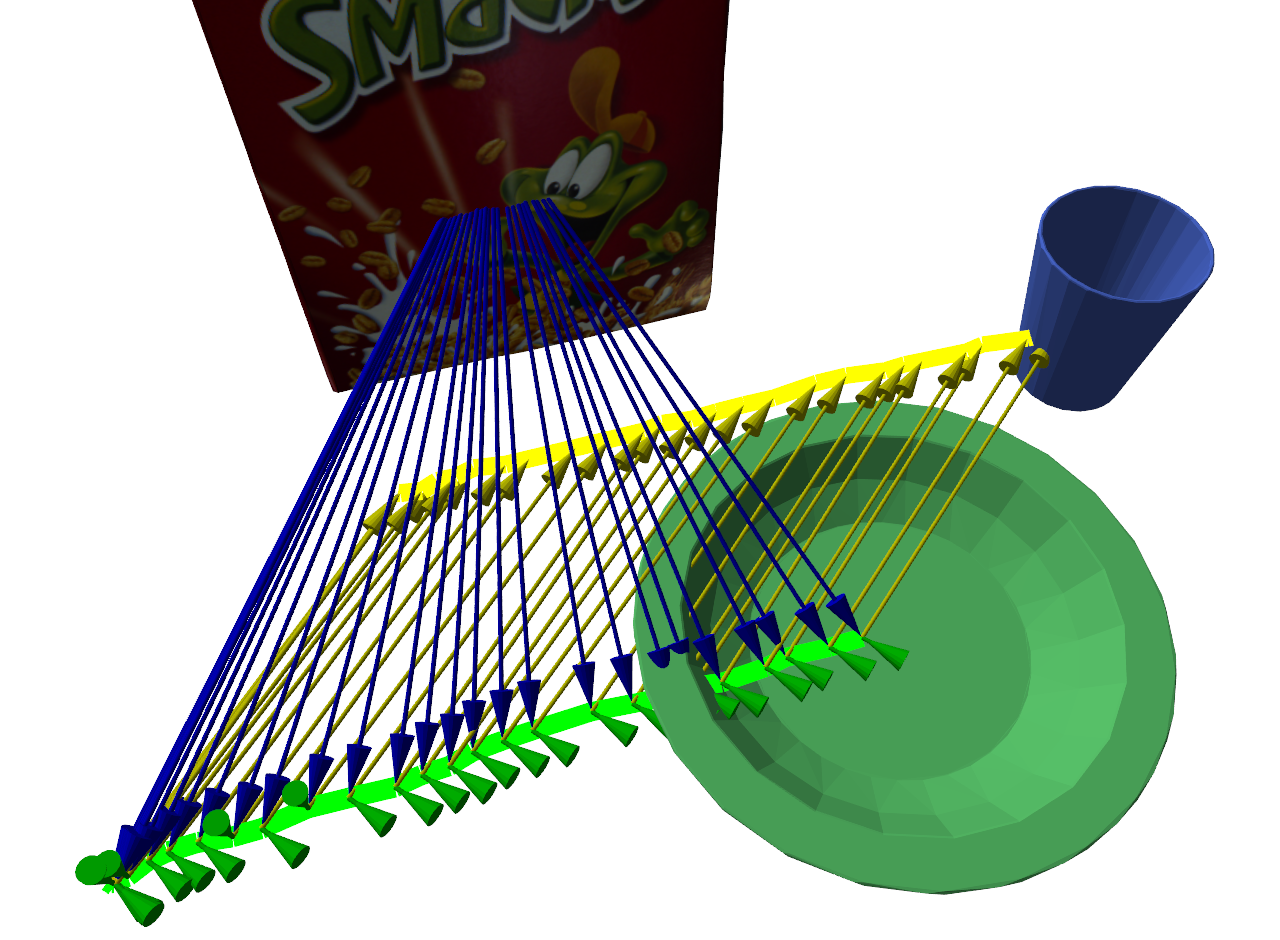
\includegraphics[width=0.7\textwidth]{./bilder/paper_fotos/fruhstuck-cluster.png}
  \caption{Spuren und Votes einer trainierten Szene mit Clustering. Bildquelle: \cite{P.MeissnerandR.RecklingandR.JaekelandS.R.Schmidt-RohrandR.Dillmann2013}}\label{fig:scene-train-cluster}
\end{figure}

Für das Training wird auf die in der Aufnahmephase aufgenommenen Objektmengen zurückgegriffen.

Es besteht im Wesentlichen aus dem Clustering der Objektspuren mittels spezieller Heuristiken, gefolgt von der Bildung eines ISMs auf Basis aller nicht-clusterfähigen verbleibenden Spuren.
Der grundlegende Trainingsalgorithmus ist im Algorithmus \vref{algo:training} dargestellt.

Beispielhaft ist in Abbildung \vref{fig:scene-train-cluster} das Ergebnis des Trainings einer Scene mit Clustering zu sehen.
Da sich der Teller und der Becher immer gemeinsam bewegt haben, wurden sie durch die direktionale Heuristik geclustert. Als Referenzobjekt der Subszene wurde der Teller ausgewählt, was man an der Verbindung zwischen Cornflakespackung und Teller erkennen kann.

\begin{algorithm}
  \caption{Training}
  \label{algo:training}
  \begin{algorithmic}[1]
    \Require Objektmengenliste $M_O$, Szenenname $N$\;
    \Ensure Menge von ISMs\;
    \State Spuren $\gets$ ObjektmengenListeZuSpuren($M_O$)\;
    \State ClusterID $\gets 0$\;
    \State ISMs $\gets \{ \}$\;
    \While{True}
      \State Ergebnis $\gets$ Heuristik(Spuren)\;
      \If{Ergebnis $=$ null}
          \State break\;
      \EndIf
      \State Spur$_1$, Spur$_2$, Konfidenz $\gets$ Ergebnis\;
      \If {Konfidenz $<$ Schwellwert}
          \State break\;
      \EndIf
      \State SubSzenenName $\gets N$ + '\_sub' $+$ ClusterID\;
      \State ISM, ReferenzSpur $\gets$ TrainiereISM(\{Spur$_1$, Spur$_2$\}, SubSzenenName)\;
      \State Spuren $\gets$ (Spuren $\setminus$ \{Spur$_1$, Spur$_2$\}) $\cup$ \{ReferenzSpur\}\;
      \State ISMs $\gets$ ISMs $\cup$ \{ISM\}\;
    \EndWhile
    \State ISM, ReferenzSpur $\gets$ TrainiereISM(Spuren, N)\;
    \State \Return ISMs $\cup$ \{ISM\}\;
  \end{algorithmic}
\end{algorithm}

\section{Erkennung}

\begin{algorithm}
  \caption{Erkennung einer Szene}
  \small\label{algo:erkennung-main}
  \begin{algorithmic}[1]
    \Require Objektmenge $O_I$\;
    \Ensure Ergebnismenge\;
    \State Durchlaufzahl $\gets 0$\;
    \State Nochmal $\gets$ False\;
    \Repeat
      \State Ergebnis, $O_I$, Nochmal $\gets$ Erkennungsrunde mit $O_I$\;
      \State Durchlaufzahl $\gets \text{Durchlaufzahl} + 1$\;
    \Until{$\text{Durchlaufzahl} > \text{MaxDurchlaufZahl} \vee \text{Nochmal} = \text{False}$}
    \State \Return Ergebnis\;
  \end{algorithmic}
\end{algorithm}

Die Wiedererkennung bereits gelernter Szenen stellt den komplexesten Teil des Verfahrens dar.
Hier wird versucht aus den im Training berechneten Votes zusammen mit den Eingabedaten aus den Objekterkennern einen Rückschluss auf die betrachtete Szenen zu ziehen.

Der grundlegenden Ablauf der Erkennung ist in Algorithmus \vref{algo:erkennung-main} dargestellt.
Dabei wird die Erkennung wiederholt ausgeführt bis entweder ein Limit an Durchläufen überschritten wurde oder aus der Erkennungsrunde keine neuen Informationen mehr gewonnen werden können.
Dieses iterative Verfahren ist notwendig, da die im Training hierarchisch aufeinander aufbauenden Zusammenhänge nicht in einem Durchlauf erkannt werden können.
Stattdessen werden beim ersten Durchlauf nur Teilaspekte der Szene erkannt, welche dann wieder in die Eingabemenge eingefügt werden und als Basis für die nächsthöhere Hierarchiestufe dienen.

\subsection{Erkennungsrunde}

In der Erkennungsrunde werden die Votes auf die Eingabeobjekte angewandt, die Ergebnisse aggregiert und die Ergebnisse, zusammen mit einer veränderten Eingabemenge und einem Indikator, ob eine wiederholte Ausführung weitere Informationen liefern könnte, zurückgegeben.

Da das Anwenden der Votes für jede zu erkennende Szene separat geschieht, wird zuerst eine Hashtabelle \textit{SzenentypZuVotes} erstellt, in der die zu aggregierenden angewendeten Votes nach Szenennamen gruppiert werden.
In dieser Hashtabelle wird der Szenenname als Schlüssel und jeweils eine Menge angewandter Votes als Wert benutzt.
Auch wird eine Indikatorvariable \textit{Nochmal} benötigt, um bei der Rückgabe eine zu wiederholende Anwendung des Algorithmus zu indizieren.
Im ersten Schritt des Verfahrens wird über alle Eingabeobjekte $o$ der Eingabemenge $I$ iteriert.
Sollte das betrachtete Objekt aus der Eingabemenge bereits einen erkannten Typ haben, wird dieser als einziger Typ in die Menge \textit{Typen} eingefügt.
Sollte jedoch kein Objekttyp erkannt worden sein, werden alle bekannten Objekttypen aus der Datenbank entnommen und in die Menge eingefügt.
Dann wird über alle Typen $t$ in \textit{Typen} iteriert.
Es wird geprüft ob das Eingabeobjekt $o$ einen erkannten Objektidentifikator trägt.
Sollte dies der Fall sein, werden aus der Datenbank alle Votes gelesen, welche den Objekttyp $o.\text{Typ}$ und den Objektidentifikator $o.\text{ID}$ tragen.
Sollte das Objekt $o$ keinen erkannten Identifikator aufweisen, werden sämtliche Votes für den passenden Objekttyp geladen.
Die Votes werden in der Variable \textit{Votes} gespeichert.
Nun wird über jedes Vote $v$ aus \textit{Votes} iteriert.
Zunächst muss die Szenendefinition für den in $v$ enthaltenen Szenennamen in die Variable \textit{Szene} geladen werden.
Dann wird der Variablen \textit{Referenzpose} das Ergebnis der Anwendung des Votes auf die Objektpose $o.\text{Pose}$ zugewiesen.
Dies repräsentiert die erwartete Position und Orientierung des Referenzpunktes aus Sicht des Objektes für dieses Vote.
Aus diesen Daten wird ein angewandtes Vote $V$ erstellt, welches die Refernzpose, die Votedefinition $v$, das Ausgangsobjekt $o$ sowie das sich aus Objekt und Szene ergebende Gewicht enthält.
Das angewandte Vote wird dann in die Hashtabelle in die zum Szenennamen gehörende Menge eingefügt.
Dies schließt den ersten Schritt des Algorithmus ab.

Der zweite Schritt beschäftigt sich mit der Aggregation der angewandten Votes und ist ebenfalls essentiell für den Aufbau der Szenenhierarchien.
Dafür wird über die \textit{SzenentypZuVotes} Hashtabelle iteriert, wobei der Szenenname der Variable \textit{SName} und die Votemenge der Variable \textit{V} zugewiesen wird.
Dann wird wie in Abschnitt \vref{ch:aggregation} und Abschnitt \vref{ch:einpassung} beschrieben eine Aggregation, Einpassung und Rückprojektion mit den Votes aus $V$ durchgeführt, woraus sich die Ergebnismenge \textit{Ergebnisse} ergibt.
Daraufhin wird über jedes \textit{Ergebnis} in \textit{Ergebnisse} iteriert.
Sollte es in der Datenbank einen Objekttyp mit dem Namen der erkannten Szene \textit{Ergebnis.Szenenname} geben, so wird für das Ergebnis ein neues Objekt für die Eingabemenge generiert, welches diese Subszene repräsentiert.
Dafür bildet man ein neues Objekt \textit{RefObjekt} welches als Objekttyp den erkannten Szenennamen trägt.
Als Pose des neuen Objektes wird die Referenzpose der erkannten Subzene gewählt.
Die Konfidenz der erkannten Subszene geht direkt in die Konfidenz des neuen Objektes über.
Das Gewicht des Objektes wird aus der Summe der Gewichte aller in der Subszene erkannten Objekte berechnet.
Zur Modifikation der Eingabemenge $I$ muss zunächst überprüft werden, ob es in $I$ bereits ein Objekt mit identischem Typ, Identifikator und identischer Pose wie \textit{RefObjekt} gibt.
Sollte dies erfüllt sein und die Konfidenz oder das Gewicht des vorhandenen Objektes kleiner sein, als das von \textit{RefObjekt}, so wird das vorhandene Objekt durch \textit{RefObjekt} ersetzt.
Sollte in $I$ jedoch kein Objekt mit identischem Type, Identifikator und identischer Pose vorhanden sein, so wird \textit{RefObjekt} der Menge $I$ hinzugefügt.
In beiden Fällen wurde die Eingabemenge verändert und somit besteht die Chance, dass sich die Erkennung in einem weiteren Durchlauf mit der veränderten Eingabemenge verbessert, daher wird der Indikator \textit{Nochmal} auf \textit{True} gesetzt.
Am Ende der Schleife wird \textit{Ergebnis} der Endergebnismenge hinzugefügt.
Wurden alle Schleifen durchlaufen, gibt der Algorithmus die Endergebnismenge, die veränderte Eingabemenge sowie den Wiederholungsindikator zurück.

\begin{algorithm}
  \caption{Erkennungsrunde}
  \small\label{algo:erkennung-runde}
  \begin{algorithmic}[1]
    \Require Objektmenge $I$\;
    \Ensure Ergebnismenge, ergänzte Eingabemenge, Wiederholungsindikator\;
    \State SzenetypZuVotes $\gets$ \parbox[t]{\dimexpr\linewidth-1\algorithmicindent\relax}{Hashmap mit Szenentyp als Schlüssel und Votemenge als Wert}\strut\;
    \State Nochmal $\gets$ False\;
    \ForAll{$o \in I$}
      \State Typen $\gets \begin{cases}
          \{o.\text{Typ}\} & \text{if } o.\text{Typ} \neq \text{null}\\
          \text{Alle Objekttypen aus der Datenbank} & \text{sonst}
        \end{cases}$\;
        \ForAll{$t \in \text{Typen}$}
          \State Votes $\gets \begin{cases}
                                \text{Votes aus Datenbank mit Typ } t & \text{if } o.\text{ID} = \text{null}\\
                                \text{Votes aus Datenbank mit Typ } t \text{ und ID } o.\text{ID} & \text{if } o.\text{ID} \neq \text{null}\\
                              \end{cases}$\;
          \ForAll{$v \in \text{Votes}$}
            \State Szene $\gets$ Szenendefinition aus der Datenbank für $v.\text{Szenenname}$\;
            \State Referenzpose $\gets$ Wende Vote auf Objektpose $o.\text{Pose}$ an\;
            \State $V \gets $ \parbox[t]{\dimexpr\linewidth-1\algorithmicindent\relax}{Angewandtes Vote mit:\\
              Pose $\gets$ Referenzpose\\
              VoteDefinition $\gets v$\\
              Ausgangsobjekt $\gets o$\\
              Gewicht $\gets o.\text{Gewicht} / \text{Szene}.\text{ErwartetesGewicht}$ }\strut\;
            \State Füge $V$ in SzenentypZuVotes[Szene.name] ein\;
          \EndFor
        \EndFor
    \EndFor
    \State EndErgebnisse $\gets \{\}$\;
    \ForAll{SName, $V \in$ SzenentypZuVotes}
      \State Ergebnisse $\gets$ Aggregation, Einpassung und Rückprojektion mit $V$\;
      \ForAll{Ergebnis $\in$ Ergebnisse}
        \If{Objekt in Datenbank mit Typ $=$ Ergebnis.Szenenname}
          \State RefObjekt $\gets$ \parbox[t]{\dimexpr\linewidth-1\algorithmicindent\relax}{Neues Objekt mit:\\
            Typ $\gets$ Ergebnis.Szenenname\\
            Pose $\gets$ Ergebnis.Referenzpose\\
            Konfidenz $\gets$ Ergebnis.Konfidenz\\
            Gewicht $\gets \sum \{ o.\text{Gewicht} : o \in \text{Ergebnis}.\text{Objekte} \}$}\strut\;
          \If{Objekt $o_i$ in $I$ mit gleichen Typ$/$ID$/$Pose wie RefObjekt und\\ \hskip\dimexpr1\algorithmicindent\relax kleinerem Gewicht oder Konfidenz}
            \State Ersetze $o_i$ in $I$ mit RefObjekt\;
            \State Nochmal $\gets$ True\;
          \ElsIf{Kein Objekt $o_i$ in $I$ mit gleichen Typ$/$ID$/$Pose}
            \State Füge RefObjekt in $I$ ein\;
            \State Nochmal $\gets$ True\;
          \EndIf
        \EndIf
        \State Füge Ergebnis in EndErgebnisse ein\;
      \EndFor
    \EndFor
    \State \Return EndErgebnisse, $I$, Nochmal\;
  \end{algorithmic}
\end{algorithm}

\subsection{Aggregation}\label{ch:aggregation}

In der Aggregationsphase werden alle angewendeten Votes in einen diskretisierten dreidimensionalen Votingraum eingefügt.
Die Diskretisierung wird dabei über ein Voxelgrid realisiert.
Dazu wird über jedes Vote in der Votingmenge iteriert und die x/y/z-Koordinate jedes Votes durch eine vorher festgelegte Bucketgröße geteilt.
Dabei wird die ganzzahlige Division verwendet und die Nachkommastellen verworfen.
Das Vote wird dann in den entsprechenden Bucket eingebracht.

\begin{figure}
  \centering
  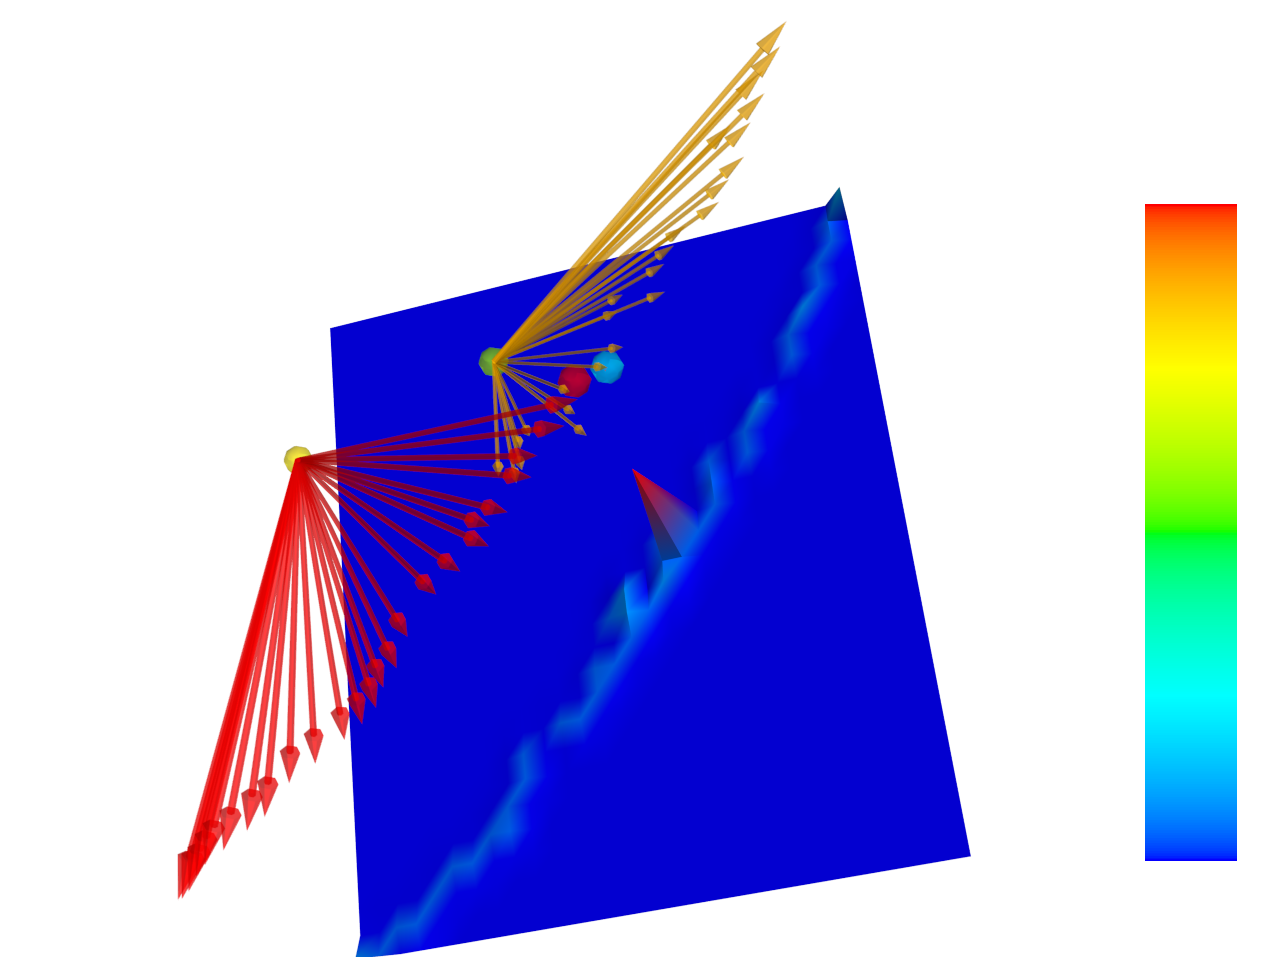
\includegraphics[width=.7\textwidth]{./bilder/paper_fotos/voting-nocluster-neu.png}
  \caption{Aggregation der Votes zweier Objekte. Bildquelle: \cite{P.MeissnerandR.RecklingandR.JaekelandS.R.Schmidt-RohrandR.Dillmann2013}}\label{fig:vote-aggr}
\end{figure}

Eine Projektion des Aggregationsvorgangs auf ein zweidimensionales Voxelgrid ist in Abbildung \vref{fig:vote-aggr} dargestellt.
Zu sehen darin sind zwei votenden Objekte zusammen mit einem Peak an der Position an die beide Objekte gleichzeitig voten.

Exemplarisch wird eine Bucketgröße von $5$ festgelegt und ein Vote an der Position $(4, 6.8, 9)$ betrachtet, dann wird dieses Vote dem Bucket an der Position $(0, 1, 1)$ zugeordnet.

\subsection{Einpassung und Rückprojektion}\label{ch:einpassung}

Die Einpassung und Rückprojektion stellt die eigentliche Szenenerkennung dar.
Sie wird jeweils mit dem Inhalt eines Buckets ausgeführt und liefert als Rückgabewert einen Szenenvorschlag.
Das Verfahren besteht aus zwei Schritten:
Der Auswahl eines Referenzpunktkandidaten, welcher für den Einpassungsversuch genutzt werden soll und dem eigentlichen Einpassungsdurchlauf, welcher als zentrale Komponente die Rückprojektion beinhaltet.
Die Auswahl des Referenzpunktkandidaten und der Aufruf der Einpassungsfunktion sind in Algorithmus \vref{algo:referenzwahl} dargestellt.

\subsubsection{Referenzwahl}

\begin{algorithm}
  \caption{Referenzpunktauswahl und Einpassungsversuch}
  \small\label{algo:referenzwahl}
  \begin{algorithmic}[1]
    \Require Angewandte Votemenge $V$\;
    \Ensure Ergebnisvorschlag\;
    \State $V \gets$ sortiere Votes in $V$ absteigend nach Konfidenz\;
    \ForAll{$v \in V$}
      \State Einpassung $\gets$ Passe Votes ein für \parbox[t]{\dimexpr\linewidth-1\algorithmicindent\relax}{
        Votemenge $\gets V$\\
        Referenzvote $\gets v$
      }\strut\;
      \If{Einpassung $\neq$ null}
        \State Konfidenz $\gets 0$\;
        \State Objektmenge $\gets \{\}$\;
        \ForAll{$v_e \in \text{Einpassung}.\text{Votes}$}
          \State Konfidenz $\gets$ Konfidenz $+$ $v_e.\text{Gewicht}$\;
          \State Erstelle eine Objektkopie $o$ aus $v_e.\text{Ausgangsobjekt}$\;
          \State $o.\text{Typ} \gets v_e.\text{VoteDefinition}.\text{Typ}$\;
          \State $o.\text{ID} \gets v_e.\text{VoteDefinition}.\text{ID}$\;
          \State Füge $o$ in Objektmenge ein\;
        \EndFor
        \State \Return Neues \parbox[t]{\dimexpr\linewidth\relax}{Erkennungsergebnis mit:\\
          Objekte $\gets$ Objektmenge\\
          Referenzpose $\gets v.\text{Pose}$\\
          Szenenname $\gets v.\text{Szenenname}$\\
          Konfidenz $\gets$ Konfidenz}\strut\;
      \EndIf
    \EndFor
    \State \Return null\;
  \end{algorithmic}
\end{algorithm}

Dabei werden die angewandten Votes aus der Eingabemenge $V$ erst nach Gewicht sortiert.
Dies ist damit zu begründen, dass das wichtigste Vote als bester Kandidat für einen Referenzpunkt gesehen wird, was aus der Tatsache folgt, dass ein höheres Objektgewicht äquivalent ist, zu einer größeren Menge an unterstützenden Objekten, welche in einer Hierarchie unterhalb des betrachteten Objektes existieren.
Nach der Sortierung wird die Einpassung der restlichen Objekte relativ zum Referenzvote $v$ vorgenommen.
Sollte diese Einpassung ein erfolgreiches Ergebnis liefern, so wird dieses Ergebnis in ein Erkennungsergebnis konvertiert.
Dazu wird über jedes erfolgreich in das Modell eingepasste Vote iteriert.
Die Konfidenz des Votes wird zur Konfidenz des Erkennungsergebnisses addiert, welche mit "`0"' initialisiert wurde.
Dann wird eine Kopie des Ausgangsobjektes erstellt und mit dem Typ und dem Identifikator des Votes annotiert.
Dies behandelt den Sonderfall, in dem der Objekterkenner dem Ausgangsobjekt keinen Typ oder Identifikator zugewiesen hat, dieser aber durch die Einpassung des Votes inferiert werden konnte.
Das modifizierte Objekt wird dann der Objektmenge des Erkennungsergebnisses hinzugefügt.
Nach der Iteration wird das Erkennungsergebnis, bestehend aus den generierten Objekten, der Referenzpose des Votes $v$, dem Szenennamen des Votes und der errechneten Konfidenz, zurückgegeben.
Sollte die Einpassung nicht erfolgreich sein, wird die Schleife weiter durchlaufen, um Referenzposen anderer Votes zu testen.
In dem Fall, dass alle Votes kein hinreichendes Einpassungsergebnis erzeugen, wird \textit{null} zurückgegeben, um eine gescheiterte Erkennung zu indizieren.

\subsubsection{Einpassung}

\begin{algorithm}
  \caption{Einpassung}
  \small\label{algo:fitting}
  \begin{algorithmic}[1]
    \Require Angewandte Votemenge $V$, Referenzvote $v_r$\;
    \Ensure Ergebnisvorschlag\;
    \State Gewählt $\gets \{v_r.\text{Ausgangsobjekt}\}$\;
    \State EingepassteVotes $\gets \{v_r\}$\;
    \ForAll{$t \in \{v.\text{VodeDefinition}.\text{Typ} | v \in V\}$}
      \State IDs $\gets \{v.\text{VodeDefinition}.\text{ID} | $ \parbox[t]{\dimexpr\linewidth\relax}{$v \in V \wedge$\\
          $v.\text{VoteDefinition}.\text{Typ} = t \wedge$\\
          $(v.\text{VoteDefinition}.\text{Typ} \neq v_r.\text{VoteDefinition}.\text{Typ} \wedge$\\
          $v.\text{VoteDefinition}.\text{ID} \neq v_r.\text{VoteDefinition}.\text{ID})\}$}\strut\;
      \ForAll{ID $\in$ IDs}
        \State Votes $\gets \{v | $\parbox[t]{\dimexpr\linewidth\relax}{$v \in V \wedge v.\text{VoteDefinition}.\text{Typ} = t \wedge$\\
            $v.\text{VoteDefinition}.\text{ID} = \text{ID}\}$}\strut\;
        \ForAll{$v \in \{v|v\in Votes \wedge v.\text{Ausgangsobjekt} \notin \text{Gewählt}\}$}
          \State ProjizierterPunkt $\gets$ Rückprojektion von $v_r.\text{Pose}$ mittels $v$\;
          \State Distanz $\gets$ \parbox[t]{\dimexpr\linewidth-1\algorithmicindent\relax}{Distanz zwischen ProjizierterPunkt und $v.\text{Ausgangsobjekt}.\text{Pose}.\text{Punkt}$}\strut\;
          \State Winkel $\gets$ Winkel zwischen den Blickvektoren von $v.\text{Pose}$ und $v_r.\text{Pose}$\;
          \If{Distanz $\leq$ Bucketgröße $\wedge$ Winkel $\leq$ MaximalerWinkelabstand}
            \State Gewählt $\gets \text{Gewählt} \cup \{v.\text{Ausgangsobjekt}\}$\;
            \State EingepassteVotes $\gets \text{EingepassteVotes} \cup \{v\}$\;
            \State break\;
          \EndIf
        \EndFor
      \EndFor
    \EndFor
    \State \Return EingepassteVotes\;
  \end{algorithmic}
\end{algorithm}

In der Einpassungsphase wird versucht die in den Bucket eingegangenen Votes im Bezug zu einem ausgewählten Referenzvote so auf die dazugehörigen Ausgangsobjekte zu verteilen, dass am Ende jedes Objekt nur ein Vote zur Szene beiträgt und die verwendeten Votes nicht im Widerspruch zu dem Modell der Szenen stehen.
Um dies zu erreichen wird jeweils ein Vote aus der Votemenge des Buckets festgehalten und mit den verbleibenden Votes eine Greedy-Suche durchgeführt, welche versucht, Votes möglichst schnell auf die beteiligten Objekte zu verteilen.
Durch diesen Ansatz ist es möglich, dass die gefundene Einpassung der Votes in das Szenenmodell nicht optimal ist, jedoch ist mit einigen Feineinstellungsparametern der Zuweisungsfehler einfach mit der Ausführungsgeschwindigkeit abzustimmen.
Der Vorgang ist in Algorithmus \vref{algo:fitting} in Pseudocode verdeutlicht.

Grundlegend versucht der Einpassungsalgorithmus jedem Ausgangsobjekt genau ein Vote zuzuweisen, sodass die Gesamtheit der zugewiesenen Votes mit dem Modell in Einklang stehen.
Dies bedeutet ferner, dass keine zwei zugewiesenen Votes die gleiche Typ/ID Kombination besitzen dürfen und dass die Positions- und Winkelabweichung der Referenzpose der gewählten Votes von der Referenzpose des im vorigen Schritt festgehaltenen Referenzvotes einen gesetzten Ungenauigkeitsschwellwert nicht überschreiten darf.

Im ersten Schritt des Verfahrens werden zwei Mengen \textit{Gewählt} und \textit{EingepassteVotes} erstellt.
Die Menge \textit{Gewählt} enthält Referenzen zu Ausgangsobjekten, welchen bereits ein Vote zugewiesen wurde. Sie ist mit dem Ausgangsobjekt des Referenzvotes initialisiert.
Die Menge \textit{EingepassteVotes} beinhaltet die bereits verteilten Votes.
In der ersten Iteration wird über jeden Objekttyp $t$ iteriert, welcher in der Votemenge $V$ enthalten ist.
Innerhalb dieser Schleife wird die Menge \textit{IDs} erzeugt, welche alle IDs enthält, die in Votes des Typs $t$ auftauchen.
Dabei wird die Typ/ID-Kombination des Referenzvotes ausgelassen, da dieses schon in der Ergebnismenge enthalten ist.
Darauf folgend wird über jede \textit{ID} in \textit{IDs} iteriert.
Innerhalb dieser Schleife wird zunächst die Variable \textit{Votes} definiert.
Die Menge \textit{Votes} besteht aus allen Votes aus $V$ mit dem Typ \textit{t} und der ID \textit{ID}.
Über diese Votemenge wird nun ebenfalls über jedes Vote $v$ iteriert, wobei in jedem Schleifendurchlauf zusätzlich geprüft wird, ob das Ausgangsobjekt für das zu betrachtende Vote bereits vergeben ist.
Sollte dies das Fall sein, wird das betreffende Vote übersprungen.
Innerhalb der Voteiteration wird die eigentliche Rückprojektion durchgeführt.
Zunächst wird versucht anhand der Pose des Referenzvotes und der Rücktransformation des Votes $v$ auf den Ursprungspunkt \textit{ProjizierterPunkt} des Ausgangsobjektes zurückzuschließen.
Daraus wird die Abweichung \textit{Distanz} zwischen dem projizierten und dem echten Ursprungspunkt aus dem Ausgangsobjekt von $v$ berechnet.
Darauf folgt die Berechnung des Winkels zwischen der Orientierung der von $v$ vorgeschlagenen Referenzpose und der durch $v_r$ gewählten Referenzpose.
Dann wird geprüft, ob die Distanz kleiner oder gleich der Bucketgröße und der Winkelunterschied kleiner als \textit{MaximalerWinkelabstand} ist.
Die Bucketgröße wird dabei als generelle Sensitivität oder "`ungefähre maximale Positionsabweichung"' der Erkennung verstanden.
Es wäre in gleichem Maße möglich an dieser Stelle einen separaten frei gewählten Parameter zu verwenden, die Bucketgröße hat sich in Experimenten jedoch als ausreichend erwiesen um zuverlässige Ergebnisse zu generieren.
\textit{MaximalerWinkelabstand} ist ein weiterer frei wählbarer Parameter um die Genauigkeit des Ergebnisses gegenüber Geschwindigkeit und Sensorrauschen abzuwägen.
Dabei hat sich eine Abweichung von 10$^\circ$ als geeigneter Wert herausgestellt.
Sollen die beiden Bedingungen erfüllt werden, so wird das Ausgangsobjekt von $v$ der Mengen \textit{Gewählt} und $v$ der Menge \textit{EingepassteVotes} hinzugefügt und die Schleife verlassen.
Nachdem alle Schleifen für alle Typ/ID-Kombinationen durchlaufen wurden, wird die Menge \textit{EingepassteVotes} als Ergebnismenge zurückgegeben.
